\documentclass[acmsmall,screen,review,anonymous]{acmart}

\usepackage{amsmath}
\usepackage{array}
\usepackage{graphicx}
\usepackage{tikz}
\usepackage{xcolor}
\usepackage{xspace}
\usetikzlibrary{arrows.meta,backgrounds,calc,fit,positioning}

\setcopyright{none}
\copyrightyear{2027}
\acmYear{2027}
\acmDOI{}
\acmConference[FSE 2027]{The ACM International Conference on the Foundations
of Software Engineering}{July 12--16, 2027}{Shenzhen, China}
\settopmatter{printacmref=true,printccs=true,printfolios=true}
\renewcommand\footnotetextcopyrightpermission[1]{}
\citestyle{acmnumeric}

\newcommand{\method}{\textsc{DAP}\xspace}
\newcommand{\pds}{\textsc{PDS--ADP}\xspace}

\title[Direct Action Planning]
{Direct Action Planning: An Auditable Action-Comparison Contract for
Finite-Budget Resource Scheduling}

\author{Anonymous Author(s)}
\affiliation{\institution{Anonymous Institution}\country{Anonymous}}

\begin{abstract}
Finite-budget resource schedulers allocate capacity under uncertain demand
while reserving resources for future work. Making these decisions auditable
requires a common interface between candidate evaluation, action selection,
and resource accounting. We present Direct Action Planning (DAP), an
action-comparison contract that carries a decision's rationale through
execution. DAP constructs explicit action effects under one causal forecast,
evaluates the continuation value of affordable post-cost states, and sends the
feasible score maximizer directly to the actuator. Its decision record links
candidate consequences, resource commitments, scores, and execution receipts,
enabling independent checks across software components. We evaluate DAP on
two public workload traces, an exhaustive dynamic-programming diagnostic,
executable fault injections, and a Kubernetes implementation. On GenTD26,
explicit action effects raise completion by 3.79 percentage points and save
19.09 resource units relative to a matched learned-transition control.
The checker detects and localizes all 3,554 activated contract violations
across two value representations, with zero false positives in 640 clean
contexts and a median checking cost of 7.80 microseconds. In 160 matched
Kubernetes runs, DAP delivers every logged feasible maximizer; on Azure, it
raises completion by 6.77 points and reduces Ready-resource cost by 54.4\%
relative to immediate scoring. These results show how explicit action
semantics can support efficient resource allocation and independently
checkable execution within one scheduling interface.

\end{abstract}

\keywords{resource scheduling, finite budget, approximate dynamic programming,
action-comparable planning, Kubernetes, autoscaling}

\begin{CCSXML}
<ccs2012>
<concept>
  <concept_id>10010147.10010178.10010199</concept_id>
  <concept_desc>Computing methodologies~Planning and scheduling</concept_desc>
  <concept_significance>500</concept_significance>
</concept>
<concept>
  <concept_id>10011007.10010940.10011003.10011002</concept_id>
  <concept_desc>Software and its engineering~Software performance</concept_desc>
  <concept_significance>300</concept_significance>
</concept>
</ccs2012>
\end{CCSXML}

\ccsdesc[500]{Computing methodologies~Planning and scheduling}
\ccsdesc[300]{Software and its engineering~Software performance}

\begin{document}
\maketitle

\section{Introduction}

Resource scheduling connects software decisions to capacity. In autoscaling,
admission control, and queue management, a controller chooses a concrete
command while preserving resources for future demand. Capacity used to clear
a queue now is unavailable for a later burst. Finite-budget scheduling
therefore requires both an estimate of future opportunity and an explicit
account of what each affordable action changes. Figure~\ref{fig:motivation}
illustrates two candidate consequences: serving more work now consumes future
opportunity, whereas waiting preserves resource while accepting queue pressure.
The scheduler compares these consequences under the same remaining budget
and horizon.

\begin{figure*}[t]
  \centering
  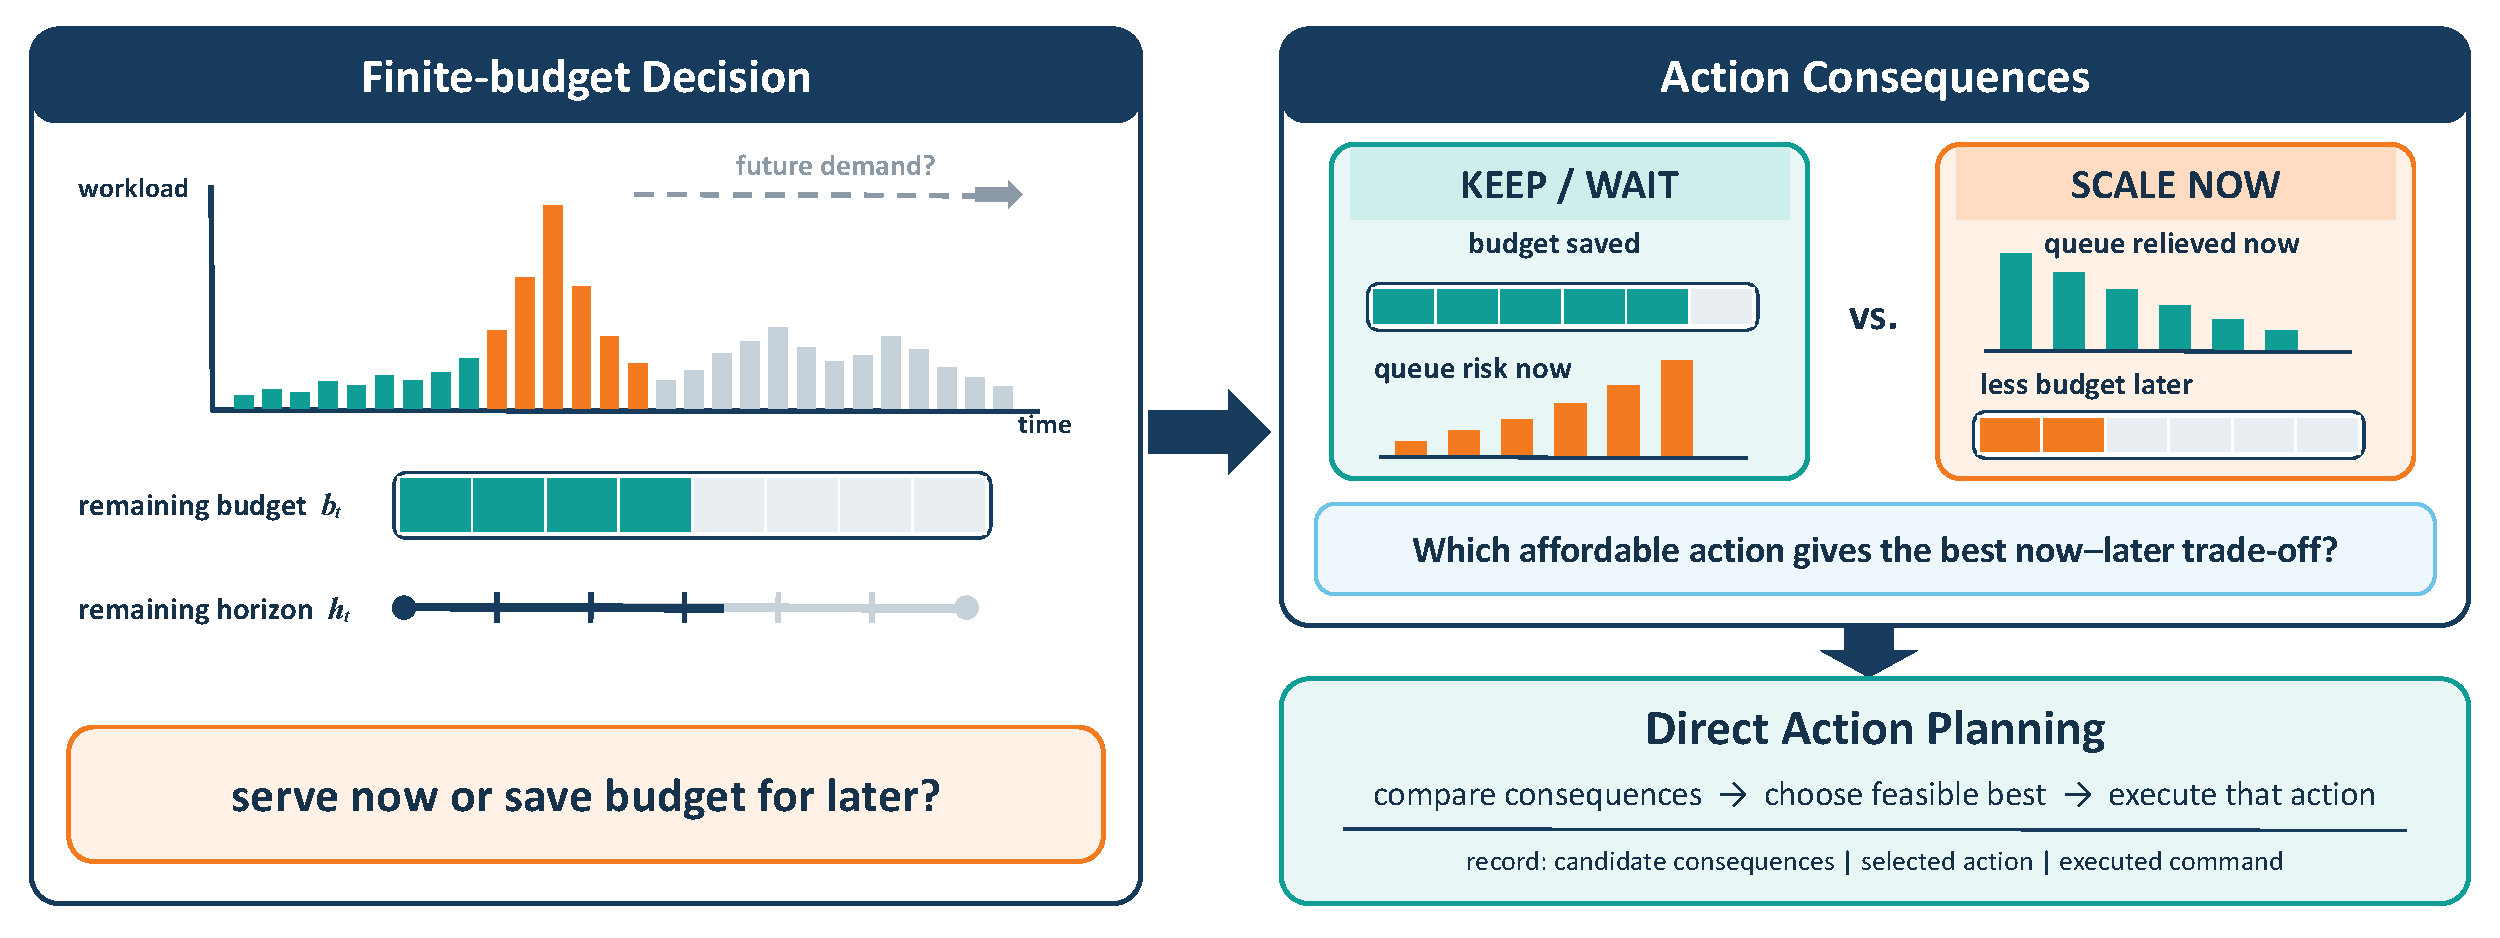
\includegraphics[width=.78\textwidth]{figures/MOTIVATION_v4.pdf}
  \caption{Motivation for direct action planning.  The schematic endpoints show
  how a lower-resource action preserves later opportunity, while a
  higher-resource action can improve current service at the cost of future
  budget.  \method compares the affordable consequences among four capacity
  levels and executes the best now--later trade-off.}
  \Description{A finite-budget decision is shown beside low- and high-resource
  action consequences.  The lower-resource endpoint preserves budget while
  accepting current queue pressure; the higher-resource endpoint relieves the
  current queue while consuming later opportunity.  Direct Action Planning
  compares affordable consequences, chooses the feasible best action, and
  executes that action.}
  \label{fig:motivation}
\end{figure*}

Deployment adds a second requirement: the choice must remain identifiable
across forecasting, value estimation, actuation, and accounting. Consider a
controller choosing among absolute replica targets. Two targets may both
satisfy a local API check and the budget, yet only one maximizes the planner's
score. Verifying execution requires connecting those scores to the delivered
command and its resource charge. An action-level record makes that
relationship observable throughout the control cycle.

Existing approaches provide complementary foundations. Model-free policies
learn long-run choices from interaction
\cite{schulman2017ppo,sutton2018rl,vanhasselt2016double}, and constrained
reinforcement learning (RL) incorporates resource costs and policy constraints
\cite{achiam2017cpo,chow2018lyapunov,stooke2020pid,tessler2019rcpo,zhang2022p3o}.
Model predictive control (MPC) exposes model structure through online
lookahead \cite{mesbah2016smpc}; post-decision-state approximate dynamic
programming (PDS/ADP) separates controlled effects from subsequent exogenous
uncertainty \cite{bhat2026pds,jiang2015monotoneadp,powell2011adp}.
Our focus is their connection to execution: candidate consequences,
affordability, scores, and actuator identity must describe the same choice.
Resource effects available as equations or calibrated API semantics provide
a basis for making that connection explicit.

We introduce Direct Action Planning (DAP), an action-comparison contract for
finite-budget scheduling. Its central idea is to make the feasible action
comparison an explicit software object. Every candidate receives one common
causal forecast; its known resource effect constructs a post-cost state;
and a learned continuation value estimates the opportunity remaining after
that action. The feasible maximizer is sent directly to the actuator. The
record binds these computations to the delivered command and measured ledger
update, enabling a checker to reconstruct the selection and localize a
disagreement at a software boundary.

Explicit effects preserve action semantics, while continuation value amortizes
longer-horizon reasoning into one-step comparisons. A PDS adapter reuses the
record with a different value representation. Two public traces, exact
dynamic programming (DP), fault injections, and Kubernetes runs evaluate these
capabilities: matched controls test service productivity and action ordering,
and independent receipts verify delivery.

The paper makes three contributions:
\begin{enumerate}
  \item \textbf{An action-comparison contract for resource scheduling.}
  We formalize a decision record that connects causal context, explicit
  candidate effects, external affordability, action scores, and execution
  identity. The contract makes feasibility, service productivity, and
  planner-to-actuator correctness separately measurable
  (Section~\ref{sec:problem}).
  \item \textbf{Efficient planning with explicit resource effects.}
  We develop a structured planner that evaluates affordable post-cost states
  with a shared forecast and budget-conditioned continuation. Matched trace
  controls and exact-DP diagnostics establish its action-ordering benefits,
  alongside sub-millisecond mean planning in the matched evaluation
  (Sections~\ref{sec:method} and~\ref{sec:mechanisms}).
  \item \textbf{Reusable verification and a deployed realization.}
  Cross-boundary checks support both DAP and PDS. A Kubernetes controller
  realizes the contract through direct actuation and independent Ready-time
  accounting. Fault injections test detection and localization; paired live
  runs demonstrate service--resource gains and command fidelity
  (Sections~\ref{sec:k8s} and~\ref{sec:deployment}).
\end{enumerate}

\section{Problem and Design Requirements}
\label{sec:problem}

\subsection{Finite-Budget Resource Scheduling}

At time \(t\), a controller observes causal system state \(s_t\), remaining
budget \(b_t\), and remaining horizon \(h_t\).  Candidate \(a\) denotes a
resource level \(C_t(a)\) for the next control interval. Service is evaluated
against a service-level objective (SLO). We distinguish three
cost objects: the branch charge \(c_t^{\mathrm{score}}(s_t,a)\) used to form the
post-action value state, a conservative commitment
\(\bar c_t(s_t,a)\) used by the pre-actuation mask, and the measured ledger
increment \(\Delta C_t^{\mathrm{led}}\) observed after actuation.  The feasible
set is
\begin{equation}
  \mathcal A_t(b_t,s_t)=
  \{a\in\mathcal A\mid \bar c_t(s_t,a)\le b_t\}.
\end{equation}
After execution, the environment returns service reward \(r_t\) and applies
\begin{equation}
  C_{t+1}^{\mathrm{led}}=C_t^{\mathrm{led}}+\Delta C_t^{\mathrm{led}},
  \quad b_{t+1}=B-C_{t+1}^{\mathrm{led}}, \quad h_{t+1}=h_t-1.
\end{equation}
The objective is the finite-horizon discounted return
\begin{equation}
  J=\mathbb E\!\left[\sum_{t=0}^{H-1}\gamma^t r_t\right],
\end{equation}
subject to hard action affordability.  In the trace environment, every
candidate satisfies
\(c_t^{\mathrm{score}}(s_t,a)=\bar c_t(s_t,a)=c(a)\).  After execution,
\(\Delta C_t^{\mathrm{led}}=c(a_t^{\mathrm{exec}})\), so the update reduces to
\(b_{t+1}=b_t-c(a_t^{\mathrm{exec}})\).  In Kubernetes these three objects
separate expected interval cost, a state-dependent safety reserve, and sampled
Ready-Pod-time consumption.  In both realizations, \(s_t,b_t,h_t\) form one
14-dimensional observation \(o_t\).

We split the transition into an action-controlled component and an exogenous
component.  Let \(g\) encode the controlled queue, capacity, service, and action-cost
effects, and let \(x_{t+1}\) denote future demand. Budget and horizon are
tracked separately.  Then
\begin{equation}
  s_{t+1}=F(s_t,a_t,x_{t+1})
  =f_{\mathrm{exo}}\!\left(g(s_t,a_t),x_{t+1}\right).
\end{equation}
The scheduling software already implements \(g\): the resource target and
action price are explicit, and an equation or calibration describes how
capacity drains a queue. This structure provides a useful division of labor.
Explicit branches compute the controlled effects, while learning estimates
exogenous demand and the continuation value of the resulting state.

The trace constraint is pathwise rather than an expected-cost objective.  With
nonnegative exact token costs, \(b_0=B\), and
\(a_t\in\mathcal A_t(b_t,s_t)\), induction gives
\(\sum_t c(a_t)\leq B\).  Value error can change which feasible action is
chosen, but it cannot authorize an unaffordable trace action.  The Kubernetes
realization retains the hard pre-actuation mask while replacing exact tokens
with a state-dependent commitment and a sampled Ready-time ledger; its
conditional bound and empirical compliance evidence are specified in
Section~\ref{sec:k8s}.

\subsection{Why Finite Budgets Require Direct Action Comparison}

The relative value of the choices in Figure~\ref{fig:motivation} depends on
remaining budget and horizon as well as current service gain. DAP makes this
comparison explicit by constructing each candidate's queue, service, and
post-cost budget before evaluating its continuation.

A shared causal forecast holds the assumed future workload fixed across
candidate branches. Together with explicit action effects, it gives each
score a concrete interpretation: immediate service plus the opportunity
remaining after this affordable action. The fields in Table~\ref{tab:state}
supply this comparison.

\begin{table}[t]
\caption{Causal observation contract used by the trace environments and the
Kubernetes controller.  Every transform is fitted on training data only.}
\label{tab:state}
\small
\begin{tabular}{p{.25\linewidth}p{.68\linewidth}}
\toprule
Group & Fields and decision role\\
\midrule
Demand & Current load, recent load, and burst intensity summarize the observed
arrival process and drive the shared next-load forecast.\\
Queue/service & Queue, queue growth, active capacity, hot-resource ratio,
utilization, mean/tail latency, SLO history, and resource pressure expose the
known effect that an action can change.\\
Opportunity & Remaining-budget and remaining-horizon ratios condition the value
of preserving resource for future decisions.\\
\bottomrule
\end{tabular}
\end{table}

\subsection{Action-Comparison Contract and Execution Fidelity}
\label{sec:requirements}

These are requirements on the deployed decision path.  They complement the
optimization objective by making affordability, action comparison, and the
actuator boundary observable in the same cycle.

\paragraph{Definition 1 (Action-comparable execution contract).}
For one causal observation \(o_t\) containing normalized budget and horizon,
let \(b_t\) also denote the corresponding raw, auditable external-ledger value.
Given common descriptor \(\widehat x_{t+1}\), the decision record is
\begin{equation}
 \begin{aligned}
 \mathcal D_t=\{&o_t,b_t,\widehat x_{t+1},
   (\bar c_t(s_t,a))_{a\in\mathcal A},\\
 & (\widehat o'_{t,a},c_t^{\mathrm{score}}(s_t,a),r_t(a))
   _{a\in\mathcal A},\\
 & (V_\theta(\widehat o'_{t,a}),Q_{\method}(o_t,a))
   _{a\in\mathcal A_t(b_t,s_t)},
   (Q_{\method}(o_t,a)=-\infty)_{a\notin\mathcal A_t(b_t,s_t)},\\
 & a_t^{\mathrm{plan}},a_t^{\mathrm{exec}},
   \Delta C_t^{\mathrm{led}},C_{t+1}^{\mathrm{led}},b_{t+1}\}.
 \end{aligned}
\end{equation}
A controller satisfies the contract when (C1) every candidate uses the same
timestamped exogenous descriptor; (C2) its explicit action effect and exact
or calibrated scoring charge construct the post-action state before
continuation value is evaluated; (C3) an external ledger applies
\(\bar c_t(s_t,a)\) and removes unaffordable candidates before
\(a_t^{\mathrm{plan}}=\arg\max_{a\in\mathcal A_t(b_t,s_t)}
Q_{\method}(o_t,a)\); and (C4) the
delivered command, observed resource use, and next ledger state are recorded so
that \(a_t^{\mathrm{exec}}=a_t^{\mathrm{plan}}\) can be checked.

Four design requirements follow: (R1) shared causal context; (R2) explicit
action effects; (R3) continuation at the post-cost budget and horizon; and
(R4) preservation of action identity through delivery and accounting.
Figure~\ref{fig:framework} maps them to planner modules. Step-keyed state,
action, and event records expose the resulting invariants for replay.

These requirements separate three properties that are often conflated.
\emph{Feasibility} asks whether a decision respects the resource ledger.
\emph{Productivity} asks how much service the consumed resource produces.
\emph{Execution fidelity} asks whether the deployed action preserves the
candidate ordering intended by the value computation:
\begin{equation}
 F_{\mathrm{exec}}=\frac{1}{T}\sum_{t=1}^{T}
 \mathbf 1\!\left[a_t^{\mathrm{exec}}=
 \arg\max_{a\in\mathcal A_t(b_t,s_t)}Q_{\method}(o_t,a)\right].
\end{equation}
Execution fidelity measures the preservation of a planned decision through
delivery. Service completion, SLO outcomes, and resource use evaluate the
quality of that decision; ledger closure and feasibility evaluate accounting.
Keeping these quantities distinct lets an evaluator locate a discrepancy in
action valuation, selection, actuation, or resource measurement. The native
interfaces in Table~\ref{tab:contract-compare} motivate bringing these
relations together in one runtime object.

\begin{table*}[t]
\caption{Native decision interfaces of common controller abstractions.
``External'' marks a field outside the method's native decision object; \method
emits candidate consequences, affordability, scores, and actuation identity as
one runtime record.}
\label{tab:contract-compare}
\scriptsize
\setlength{\tabcolsep}{3pt}
\newcolumntype{L}[1]{>{\raggedright\arraybackslash\hyphenpenalty=10000\exhyphenpenalty=10000}p{#1}}
\begin{tabular}{L{.12\textwidth}L{.22\textwidth}L{.19\textwidth}L{.18\textwidth}L{.18\textwidth}}
\toprule
Abstraction & Candidate comparison & Budget semantics & Decision artifact & Actuator boundary\\
\midrule
Learned policy controller & Policy logits or learned action values; explicit effects not intrinsic & External mask or learned constraint & Policy output & Integration layer\\
Lagrangian RL & Cost enters reward or dual update & Expected or penalized cost; hard mask external & Policy output plus multiplier & Integration layer\\
PDS/ADP & Exact controlled afterstate; exogenous effect in expectation & External constraint interface & Afterstate values & Selection and actuation may be external\\
MPC & Explicit online sequence tree under a model & Constraints inside optimizer & Plan can expose action or sequence scores & Deployment records identity of first command\\
Actor distillation & Planner supplies offline labels & Runtime mask external & Actor output can differ from teacher & Actor command\\
\method & Shared forecast plus structured action branches & External feasible set before actuation & Complete feasible score vector & Logged feasible argmax delivered directly\\
\bottomrule
\end{tabular}
\end{table*}

\section{Direct Action Planning}
\label{sec:method}

DAP combines learned exogenous demand and continuation value with explicit
resource-transition equations. Figure~\ref{fig:framework} shows how shared
context, candidate branches, post-cost scoring, and direct actuation implement
the four requirements. Measured resource feedback closes the decision loop.

\begin{figure*}[t]
  \centering
  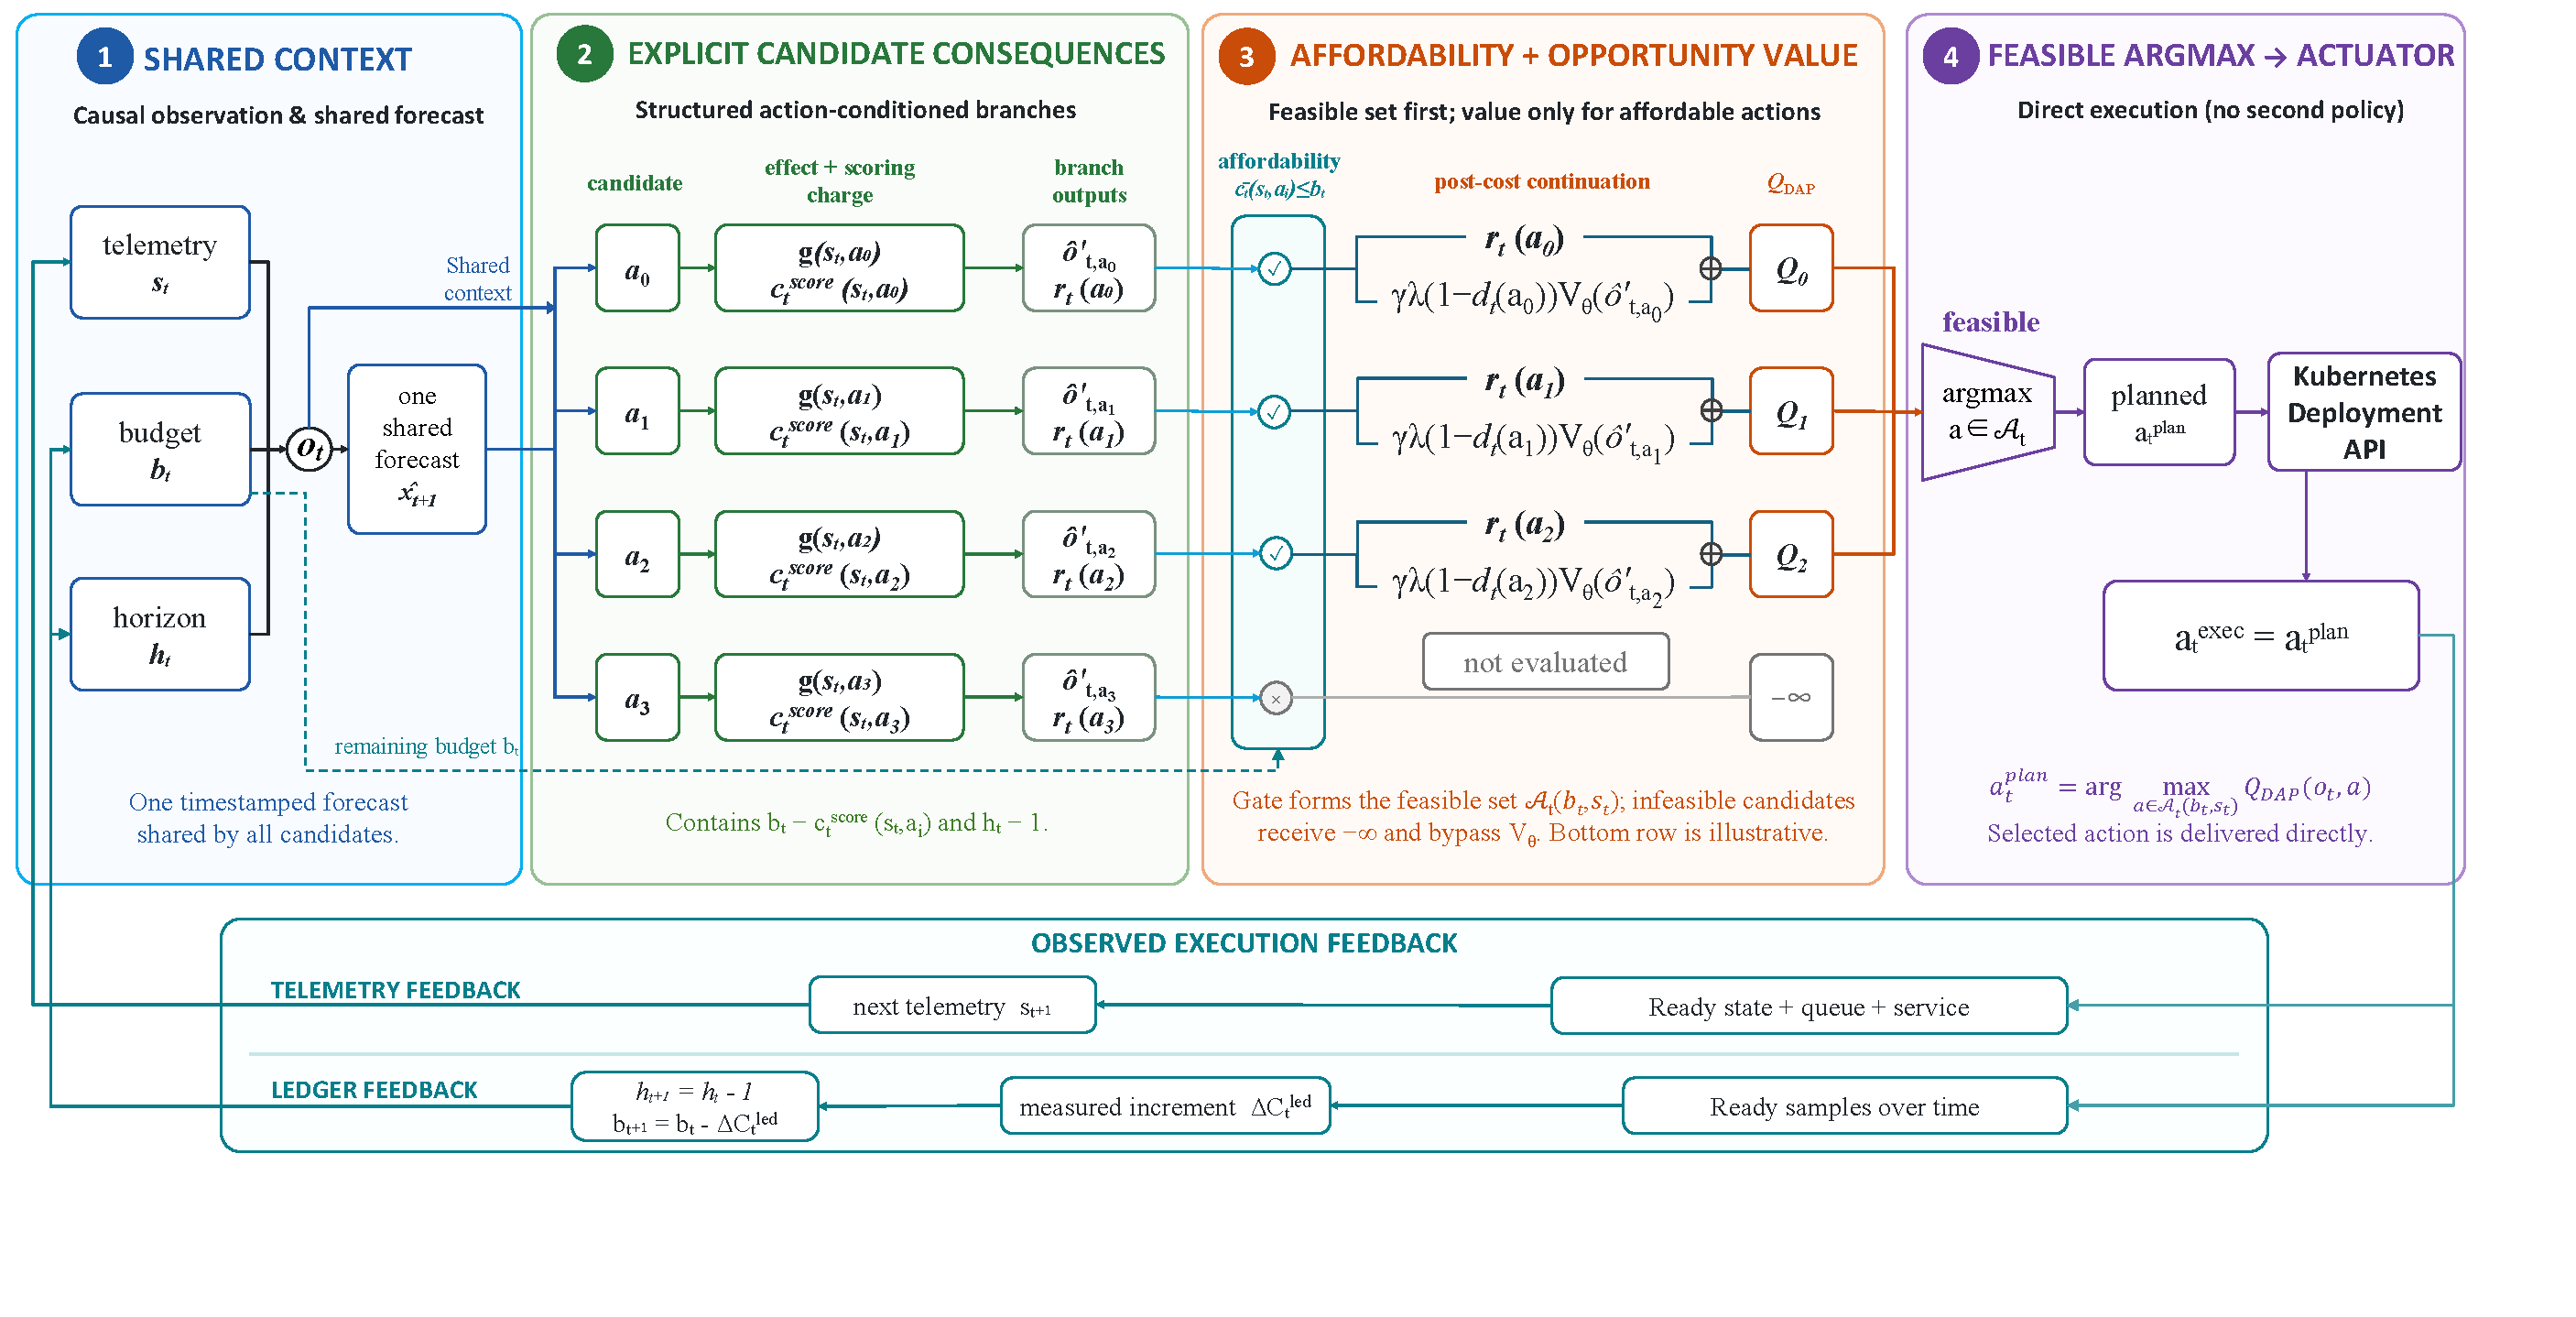
\includegraphics[width=.98\textwidth,pagebox=cropbox]{figures/FRAMEWORK_v7.pdf}
  \caption{The four-module \method action-comparison contract.  One observation
  and shared forecast feed explicit candidate consequences.  External
  commitments form the feasible set before learned continuation-value
  evaluation; the maximizer reaches the Kubernetes Deployment API directly,
  and separate telemetry and ledger feedback close the loop.}
  \Description{A four-stage closed-loop controller.  Telemetry, budget, and
  horizon form one observation and shared forecast.  Each action produces an
  explicit effect, scoring charge, post-cost state, and immediate reward.  An
  external affordability gate removes infeasible actions before the learned
  continuation-value call.  The feasible argmax reaches the Kubernetes Deployment API
  unchanged.  Execution updates causal telemetry and a cumulative measured
  resource ledger on separate feedback paths.}
  \label{fig:framework}
\end{figure*}

\subsection{Causal Context Shared across Actions}

Module 1 in Figure~\ref{fig:framework} combines causal telemetry \(s_t\),
budget \(b_t\), and horizon \(h_t\) into \(o_t=\phi(s_t,b_t,h_t)\).
Here \(\phi\) constructs the 14 features in Table~\ref{tab:state} using
training-fitted normalization. Current reward uses observed load \(x_t\);
the forecaster, with parameters \(\psi\), predicts next load once,
\begin{equation}
  \widehat x_{t+1}=f_\psi(o_t),
\end{equation}
and the same timestamped value is supplied to every candidate action.  The
action-invariant forecaster receives all 14 causal features and uses a
\(14\!\rightarrow\!32\!\rightarrow\!32\!\rightarrow\!1\) Tanh network with
non-negative output.  Training minimizes
\(\mathcal L_{\mathrm{load}}+4\mathcal L_Q+2\mathcal L_{\mathrm{rank}}\):
Smooth-L1 log-load error, normalized feasible-branch Q error, and pairwise
ranking loss with margin 0.02.  Validation selects the epoch by action error
plus 0.25 normalized Q error and 0.05 load error.
The value is fitted first and frozen during 24 forecast-training epochs.
For training state \(j\), targets
\mbox{\(Q_j^\mathrm{target}(a)=r_j(a)+\gamma(1-d_j)V_\theta(o'_{j,a})\)}
use observed next-load branches; predictions substitute the common forecast.
The recorded terminal bit is \(d_j\).
\(\mathcal L_Q\) is Smooth-L1 error after dividing both Q vectors by the
training feasible-Q standard deviation (floored at one).
\(\mathcal L_{\mathrm{rank}}\) is the pairwise hinge loss on normalized
Q differences, with the target ordering supplying the sign. Adam uses
learning rate \(10^{-3}\), batches of 256, and gradient clipping at 5.

The shared forecast implements R1; its recorded timestamp supports independent
checks of causal context across all branches.

\subsection{Explicit Action-Conditioned Transitions}

The trace action is a one-step capacity level, not a persistent increment:
\(C_t(a)=C_{\mathrm{base}}+\delta(a)\), with token costs
\((0,1,2,4)\) and nominal extras \((0,1,2.2,4.8)\).  The effect lasts for the
current trace step and the next decision chooses a fresh level.  Dataset-specific
capacity calibration is fitted on training data and shared by all methods.  In
the Kubernetes instantiation the same ordered action identifiers map instead
to absolute Deployment targets \((1,2,3,5)\), which persist until the next
command; its \texttt{no\_op} identifier denotes the base/recovery target
1, so it requests scale-down when the current target is larger.  For current arrival \(x_t\),
queue \(q_t\), and candidate capacity \(C_t(a)\), each copied branch applies
\begin{align}
  u_t &= q_t+x_t, & y_t(a)&=\min(u_t,C_t(a)),\\
  q_{t+1}(a)&=\operatorname{clip}(u_t-y_t(a),0,q_{\max}),
\end{align}
followed by per-step clearance, a queue-derived latency proxy, and its SLO indicator:
\begin{align}
  \rho_t(a)&=\frac{y_t(a)}{\max(u_t,1)},\\
  \ell_t^{\mathrm{tail}}(a)&=1+\frac{2q_{t+1}(a)}{C_t(a)},\\
  z_t(a)&=\mathbf 1[\ell_t^{\mathrm{tail}}(a)>\ell_{\mathrm{SLO}}].
\end{align}
The common simulator reward is
\begin{equation}
  r_t(a)=\rho_t(a)-0.04q_{t+1}(a)
  -0.08\ell_t^{\mathrm{tail}}(a)-2z_t(a).
\end{equation}
After inserting the shared forecast, the branch emits
\begin{equation}
  \widehat o'_{t,a}=\phi(s'_{t,a}(\widehat x_{t+1}),
  b_t-c_t^{\mathrm{score}}(s_t,a),h_t-1).
\end{equation}
Here \(s'_{t,a}(x)=f_{\mathrm{exo}}(g(s_t,a),x)\). The hat marks predicted
load; training branches \(o'_{j,a}\) use observed transitions.
Figure~\ref{fig:framework} labels candidates \(a_0,\ldots,a_3\):
\(g\) supplies their effects, and \(\phi\) inserts the updated budget and horizon.

\subsection{Affordability and Continuation Value}

A \(14\!\rightarrow\!64\!\rightarrow\!64\!\rightarrow\!1\) Tanh network learns
the continuation value \(V_\theta(o)\), with parameters \(\theta\).
For fitting state \(j\), fitted value iteration (FVI) regresses the target
\begin{equation}
  Y_j=\max_{a\in\mathcal A_j(b_j,s_j)}
  \left[r_j(a)+\gamma(1-d_j)V_{\bar\theta}(o'_{j,a})\right],
\end{equation}
where \(\bar\theta\) is the frozen preceding-round parameter vector.
Training uses 18 rounds indexed 0--17. At deployment, each affordable
candidate receives
\begin{equation}
  Q_{\method}(o_t,a)=r_t(a)+\gamma\lambda
  (1-d_t(a))V_\theta(\widehat o'_{t,a}),
  \qquad d_t(a)=\mathbf 1[h_t=1].
\end{equation}
Here \(\lambda\) weights continuation, and \(d_t(a)\) suppresses it at
the final decision. Figure~\ref{fig:framework} abbreviates
\(Q_\method(o_t,a_i)\) as \(Q_i\). Its gate uses \(\bar c_t\),
whereas \(c_t^{\mathrm{score}}\) sets the branch's post-cost budget.
These charges coincide for trace tokens; Kubernetes distinguishes them.
Unaffordable actions receive \(-\infty\) and bypass \(V_\theta\);
the masked \(a_3\) row illustrates a state-dependent outcome. Both deployed
planners bypass \(V_\theta\) at \(h_t=1\); terminal-mask tests verify that
immediate rewards determine the final scores.

Training has three non-overlapping chronological roles.  The fitting block
trains forecast and value candidates; the selection block chooses a retained
value round and \(\lambda\in\{0,0.25,0.5,0.75,1\}\); the development-evaluation
block supports information-matched controls.  The final temporal evaluator
loads a frozen checkpoint and performs inference only.  Selection retains the
immediate planner \((\lambda=0)\) as a candidate and applies fixed validation
guardrails: completion within 0.005, SLO violation within 0.01, and added cost
no greater than \(0.10B\) relative to that reference.  Eligible candidates are
ordered by return, completion, SLO, cost, and deterministic tie breaks.  These
rules freeze the operating point before evaluation.

For each fitting state, data collection copies the environment and executes
every affordable action, storing its reward, next observation, feasibility,
and terminal bit; 24 training and six validation episodes are collected per
domain.  Each FVI round freezes the preceding network as its target, computes
the four masked Bellman branches, and fits the state maximum with Smooth-L1
loss using Adam (learning rate \(10^{-3}\)), batches of 256, two epochs per
round, and gradient norm 5.  A DAP fitting state expands every affordable
branch using the known transition equations; these branch evaluations are
model computations, not additional environment interactions.  The network
width is 64, output scaling is fitted from training-reward RMS, and checkpoints
\(\{0,2,4,6,8,10,12,14,16,17\}\) are the ten prespecified rounds retained for
validation selection. Section~\ref{sec:evaluation} specifies the shared
interaction and safety protocol for comparisons with learned policies.

\subsection{Feasible Selection and Direct Actuation}

The controller executes the deterministically tie-broken feasible maximizer,
\begin{equation}
  a_t^{\mathrm{plan}}=
  \arg\max_{a\in\mathcal A_t(b_t,s_t)}Q_{\method}(o_t,a),
\end{equation}
and issues it directly, so \(a_t^{\mathrm{exec}}=a_t^{\mathrm{plan}}\),
preserving the selected candidate as the delivered command. The cycle record
in Definition~1 includes step-keyed state, action, and event entries with raw
and normalized observations, field timestamps, missing-data policies, branch
charges, feasible bits, API latency, and sampled ledger intervals. Replay
checks shared context, post-cost states, feasible argmax, target mapping,
delivery identity, selected-action feasibility, and ledger closure.
Figure~\ref{fig:framework} shows separate feedback for telemetry \(s_{t+1}\)
and measured cost \(\Delta C_t^{\mathrm{led}}\). Its update
\(b_{t+1}=b_t-\Delta C_t^{\mathrm{led}}\) is equivalent to the cumulative
ledger equation in Section~\ref{sec:problem}.

For \(|\mathcal A|=4\), online work is one forecast plus
\(O(|\mathcal A|)\) one-step transition and value calls.  A depth-\(K\),
width-\(W\) beam MPC performs \(O(KW|\mathcal A|)\) branch expansions.  \method
amortizes longer-horizon reasoning into \(V_\theta\) while preserving explicit
one-step action semantics and exposing an action-specific consequence trace.
Section~\ref{sec:k8s} maps
this module to a Kubernetes Deployment actuator and an independently measured
Ready-Pod-time ledger.

\paragraph{Relation to post-decision value.}
PDS/ADP separates the controlled afterstate from subsequent exogenous
uncertainty \cite{jiang2015monotoneadp,bhat2026pds}. DAP carries this
decomposition through deployment by retaining candidate effects, affordability,
scores, and actuator identity in one record. This makes the comparison
executable and replayable. Section~\ref{sec:pds} tests a matched PDS/ADP
representation, and Table~\ref{tab:contract-compare} identifies the exposed
runtime artifacts.

\section{Kubernetes Realization}
\label{sec:k8s}

The Kubernetes realization maps the contract to three concrete interfaces:
telemetry supplies causal state, the Deployment API receives absolute resource
targets, and an independent Ready-time ledger measures consumption. We
implement \method as an external Python controller for a local cluster.  Each 5-second cycle reads Deployment status, Pod readiness,
per-Pod Prometheus counters, queue depth, request rate, latency, CPU, SLO, and
remaining budget.  The planner maps its four actions to absolute replica
targets \(\{1,2,3,5\}\) and issues a Deployment scale request through
\texttt{kubectl}.  A target remains in force until the next cycle; the
``no-op'' identifier is explicitly the base/recovery action, not a hold-current
command.  Thus a base action
issued from target 5 requests scale-down.  The controller does not modify the
application or Kubernetes scheduler.

The budget charges Ready replicas above one base replica. A separate tracker
samples readiness approximately every 0.25 seconds; the pre-actuation reserve
admits candidates that fit the remaining sampled ledger.  After each run, the controller
returns to the base target and continues accounting until scale-down is
observed.  Kubernetes readiness probes ensure that a new Pod is charged and
used only once it becomes Ready; Pending or non-Ready Pods are excluded from
Service traffic \cite{kubernetesprobes}, while the target-based reserve still
accounts for their possibility of becoming Ready during the next interval.
The controller uses the Deployment scale interface exposed to the native
Horizontal Pod Autoscaler (HPA) \cite{kuberneteshpa}, preceded by DAP's planner
and Ready-time ledger. It follows the controller-oriented design of Borg and
Kubernetes \cite{verma2015borg,burns2016kubernetes}.

Let \(R(\tau)\) be the Ready-replica process and let one replica be the
uncharged base capacity.  The target continuous-time cost is
\begin{equation}
 C_{\mathrm{ready}}(t)=
 \int_0^t \max(R(\tau)-1,0)\,d\tau.
\end{equation}
For observations \((\tau_k,R_k)\), the implementation records the left-step
approximation
\begin{equation}
 \widehat C_k=\sum_{j=1}^{k}
 \max(R_{j-1}-1,0)(\tau_j-\tau_{j-1}).
\end{equation}
Every sample interval and Ready count is logged, so \(\widehat C_k\) is
independently recomputable; requested replicas are logged separately.  For
control period \(\Delta\), current Ready count \(R_t\), candidate absolute
target \(n(a)\), and calibrated lifecycle guard \(G\), the mask uses
\begin{equation}
 \bar c_t(R_t,a)=(n(a)-1)_+\Delta+
 \max\{(R_t-1)_+,(n(a)-1)_+\}G.
\end{equation}
It admits a non-base target only when
\(\widehat C_t+\bar c_t(R_t,a)\le B\); the base target remains the recovery
command. The reserve is conditional on a bounded control interval and a Ready
tail covered by \(G\), including outstanding replica commitments. Under these
conditions, an admitted action plus return to base fits the remaining ledger.
The implementation measures the left-step Ready integral, so the live budget
endpoint is sampled-ledger compliance. Exact token affordability applies to
the trace environment; continuous-time accounting additionally requires
independently bounded command delays, Ready tails, and pending commitments.

The guard is calibrated from scale-up and return-to-base observations.
For each workload profile and target, the calibration takes the maximum
observed Ready-withdrawal delay, adds its sampling gap and a one-second margin,
and validates the result on separate repetitions. Section~\ref{sec:deployment}
reports these measurements and the guards used in live comparisons.

This architecture separates three concerns: live metric collection constructs
the 14-field observation with provenance; the planner ranks feasible actions;
and the actuator plus budget ledger enforce deployment and resource semantics.
The runtime uses one timestamped snapshot per cycle.  Missing Pod metrics are
retried three times, then recorded as missing and omitted from service
features if unavailable; the independent current Ready
channel is read from Deployment status and remains separate from stale learned
features in the lag fault experiment.  If the Deployment query itself fails,
the run is marked incomplete and the cleanup path requests the base target.
Consequently, service noise can affect ranking, while the Ready-Pod ledger and
pre-actuation mask remain separate from the learned score.

The live implementation preserves the learned transition semantics: the value
branch receives interval-average Ready capacity, while an independent current-
Ready channel supplies the hard affordability mask. Utilization and
exponentially weighted moving-average (EWMA)
features use the same causal windows as training.  To keep burst estimates
causal and action-comparable, the runtime computes one envelope for all actions:
\[
\widehat x_{t+1}=1.10\max\!\left(
\widehat x^{\mathrm{neural}}_{t+1},x_t,
\widehat x^{\mathrm{EWMA}}_{t+1}\right).
\]
The contract transfers across trace and Kubernetes instantiations with
dataset- and deployment-specific fitted parameters.  Trace checkpoints are fitted on each workload's training split
and frozen before temporal testing.  Kubernetes uses separate checkpoints and
an independently measured Ready-capacity/startup/scale-down calibration,
selects controller settings on chronological validation inputs, and freezes
both before live test plans.  The GenTD26 continuation coefficient is selected on disjoint validation
plans within the same state, action, branch, mask, and actuator interfaces.

Component ownership follows the same interfaces.  The workload driver
owns a frozen request plan and client-side outcomes; the worker service owns
admission, bounded queueing, CPU work, timeout accounting, and Prometheus
metrics; Kubernetes owns Pod lifecycle and Service routing; and the controller
owns state construction, planning, budget accounting, and replica patches.
Only one controller is active in a run.  A planner, checkpoint, or API failure
triggers the base-replica cleanup path and prevents the run from being marked
complete.  This separation attributes planning, actuation, and request-accounting
outcomes to the responsible component.

Observation records retain raw and normalized values, timestamps, freshness,
and missing-data policies. Tests cover transition consistency, causal inputs,
terminal values, absolute targets, stale safety data, and delivered argmax
before formal runs are admitted to analysis.

\section{Evaluation}
\label{sec:evaluation}

The evaluation examines the contract from three complementary perspectives:
service productivity, the mechanism of action comparison, and deployed
execution. These perspectives correspond to the following research questions.
\begin{description}
  \item[RQ1 --- Effectiveness:] How does DAP translate a fixed resource budget
  into service quality compared with learned scheduling policies?
  \item[RQ2 --- Mechanism:] How do explicit action effects and continuation
  value contribute to action ordering and planning efficiency?
  \item[RQ3 --- Deployment:] How does the contract support independent
  verification and effective resource control in a deployed system?
\end{description}

\subsection{Workloads and Experimental Design}

Azure Functions 2019 provides per-minute invocations in HTTP and
asynchronous domains \cite{azurefunctions2019,shahrad2020serverless}; days 1--8,
9--11, and 12--14 form train, validation, and test. GenTD26 is drawn from the
Alibaba clusterdata trace and aggregated into ten-minute serving-demand bins
\cite{lin2025gentd}; its split is 60\%/20\%/20\%. Each validation segment is further
partitioned chronologically into 40\% model validation, 30\% checkpoint
selection, and 30\% development evaluation. Clipping, normalization, and
capacity calibration use training data only. Each dataset fits its own
controller, while the shared object is the four-module contract. Temporal slices
are frozen inference re-evaluations of previously accessed project data; code,
checkpoint, and window hashes bind their provenance.

The horizon is 64, \(\gamma=0.99\), and budgets are
\(\{48,72,96,120,144\}\).  The main matrix contains two datasets, five budgets,
and ten training seeds (820--829) with five evaluation episodes per domain.
Mask-binding frequency measures how often scarcity restricts the candidate
set, alongside the zero-overspend invariant.
GenTD26's domains are text-to-image and image-conditioned serving. Every
method records zero token overspend under the common mask.

\subsection{Comparators and Statistical Analysis}

External comparators include Double DQN, PPO, PPO-Lagrangian, CPO, P3O,
Budgeted Fitted-Q, A2C, PID-Lagrangian, and a disclosed port of LCPO
\cite{vanhasselt2016double,schulman2017ppo,achiam2017cpo,stooke2020pid,zhang2022p3o,carrara2019budgeted,hamadanian2025lcpo}.
The baselines span model-free, constrained, budget-conditioned, and
context-aware learning. Each receives 102,400 environment interactions and
a 64-unit network width. Immediate planning, MPC-2/4/8, black-box transitions,
actor distillation, budget/horizon removal, and PDS/ADP are information-matched
controls. All methods share observations, interactions, actions, rewards, trace
windows, normalization, and the affordability mask; native policy and dual
losses remain unchanged. This common safety-admission protocol measures the service productivity
of choices within the same feasible action set. DAP
and MPC expose computable effects, while model-free methods infer them. Frozen
manifests record optimizer settings, update counts, search ranges, branch
counts, and wall-clock summaries.

The trained seed is the trace unit. We use 20,000 paired seed-block bootstrap
resamples for 95\% intervals, paired Cohen's \(d_z\), wins/ties/losses,
two-sided Wilcoxon tests, and Benjamini--Hochberg correction
\cite{arcuri2011statistics,agarwal2021precipice,benjamini1995fdr}; cost matching
stays within observed budget frontiers. Kubernetes uses paired request plans,
paired-bootstrap intervals, exact sign-flip tests, and the registered Holm
family, retaining all seeds and failures. Matched trace, learned-transition,
and same-initialization feature controls use exact sign flips and Holm families of
24, 16, and eight endpoints; the matched live family contains 18 endpoints.
Budgets are averaged within each of ten paired seed or plan blocks. The
matched studies enumerate all $2^{10}$ sign assignments and use bootstrap
seed 20261002; intervals are pointwise and tests carry familywise correction.

\subsection{Measures and Reproducibility}

Return is the optimization objective. Episode completion is
\(\sum_t y_t/\max(\sum_t x_t,1)\), whereas \(\rho_t\) is the per-step
clearance term used only in reward. With initial queue zero, overflow
\(w_t=(q_t+x_t-y_t-q_{t+1})_+\) makes the conservation identity
\(\sum_t x_t=\sum_t y_t+\sum_t w_t+q_H\) explicit; unfinished and dropped
work are not completions. Trace latency and SLO are queue-model proxies,
not measured request percentiles. Kubernetes completion counts successful
HTTP requests over all scheduled requests; latency percentiles condition on
successful responses. The matched live study also reports the fraction
of all requests that fail or exceed the SLO, counting fast failures as violations.
Trace tables average episodes equally, assigning zero completion to zero-demand
episodes (0/500 Azure and 20/500 GenTD26 episodes per method). A descriptive
request-weighted check gives DAP completion 96.82\%/79.56\%; GenTD26 additionally
has 5.15\% dropped and 15.30\% unfinished arriving mass. The 5,000-episode
audit closes mass conservation to \(1.31\times10^{-12}\) and finds no token
overspend. These aggregation conventions leave the primary comparisons unchanged.
Resource
use is total action cost in the trace environment and
additional Ready-replica-seconds in Kubernetes.  We report budget utilization,
overspend, Pareto cell counts, matched-frontier effects, action disagreement,
Q-star regret, execution fidelity \(F_{\mathrm{exec}}\), and decision latency
within their corresponding evaluation families.

Frozen inference manifests bind dataset slices, configurations, checkpoints,
code, and outputs. The main trace matrix comprises 100 cells; PDS covers
100 development and 100 temporal cells. Kubernetes comparison and robustness
studies contain 260 runs; matched controls contain 160 runs and 5,120 action
records. All specified seeds and outcomes are retained with the paired
statistics defined above. Repeated steps and requests remain observations
within their seed or plan block.

\paragraph{AI-assistance disclosure.}
The authors formulated the research questions and DAP design, planned the
experiments, and interpreted the results. Under their instructions, an AI
coding assistant supported controller and adapter implementation, testing,
translation of experimental protocols into runnable scripts,
trace/GPU/Kubernetes execution, statistical and exact-DP computations from
recorded outputs, and visualization. Code, protocols, checkpoints, and
measurements retain the provenance of this assistance. The authors are
responsible for validating these artifacts and the final conclusions.

\subsection{RQ1: Service--Resource Effectiveness}

DAP produces favorable service--resource operating points on both workloads,
with the form of the gain depending on workload demand
(Table~\ref{tab:main} and Figure~\ref{fig:frontier}). On GenTD26, DAP has the best mean return,
completion, SLO violation, and cost among the compared methods. Relative to Double DQN, it
gains 45.764 return and 6.61 completion points while reducing SLO violation by
5.27 points and cost by 36.186 units. Relative to CPO, the corresponding
improvements are 57.031 return, 7.29 completion points, 6.22 SLO points, and
40.346 cost units. Every trained-seed block favors DAP, and all four corrected
comparisons have \(q=0.001953\).

\begin{table}[t]
\caption{Mean application operating points over five budgets and ten trained
seeds.  Arrows show direction; bold marks the best value in each dataset and
column, and \(\dagger\) marks a Pareto-nondominated row over all four outcomes.}
\label{tab:main}
\small
\begin{tabular}{llrrrr}
\toprule
Dataset & Method & Return $\uparrow$ & Completion $\uparrow$ & SLO $\downarrow$ & Cost $\downarrow$\\
\midrule
Azure & \method\(^{\dagger}\) & \textbf{23.783} & .9711 & \textbf{.1038} & 73.8\\
Azure & Double DQN\(^{\dagger}\) & 14.295 & \textbf{.9736} & .1186 & \textbf{62.9}\\
Azure & PPO & 6.715 & .9574 & .1967 & 91.3\\
Azure & A2C & -8.861 & .9374 & .2887 & 92.9\\
Azure & PPO-Lagrangian & 6.465 & .9561 & .2068 & 92.5\\
Azure & CPO & 20.021 & .9684 & .1200 & 86.0\\
Azure & P3O & .431 & .9551 & .2251 & 90.3\\
Azure & PID-Lagrangian & 8.033 & .9578 & .1977 & 92.2\\
Azure & Budgeted Fitted-Q & -36.729 & .9183 & .4341 & 95.9\\
Azure & LCPO & 7.833 & .9523 & .2044 & 93.8\\
\midrule
GenTD26 & \method\(^{\dagger}\) & \textbf{-105.195} & \textbf{.8851} & \textbf{.1479} & \textbf{39.0}\\
GenTD26 & Double DQN & -150.959 & .8191 & .2006 & 75.2\\
GenTD26 & PPO & -215.266 & .6979 & .2691 & 95.6\\
GenTD26 & A2C & -208.719 & .7174 & .2715 & 89.4\\
GenTD26 & PPO-Lagrangian & -222.110 & .6903 & .2716 & 96.0\\
GenTD26 & CPO & -162.225 & .8122 & .2101 & 79.4\\
GenTD26 & P3O & -221.485 & .6905 & .2711 & 96.0\\
GenTD26 & PID-Lagrangian & -219.204 & .6930 & .2706 & 96.0\\
GenTD26 & Budgeted Fitted-Q & -199.016 & .7322 & .2604 & 93.0\\
GenTD26 & LCPO & -170.505 & .7913 & .2268 & 83.0\\
\bottomrule
\end{tabular}
\end{table}

Azure exposes two operator-relevant regimes. Against CPO, DAP improves return
by 3.762 while reducing SLO violation by 1.62 points and cost by 12.144 units.
At supported cost-matched points, DAP exceeds the interpolated CPO return
frontier by 12.046 and reduces SLO violation by 5.98 points in 45/50 cells. DAP
and the cost-lean Double DQN point form distinct Pareto choices: DAP provides
higher return and lower SLO violation when additional budget is available. Against the
separately ported LCPO mechanism, all four paired outcomes favor DAP in every
trained-seed block on both datasets (\(q=0.001953\)).

\begin{figure*}[t]
  \centering
  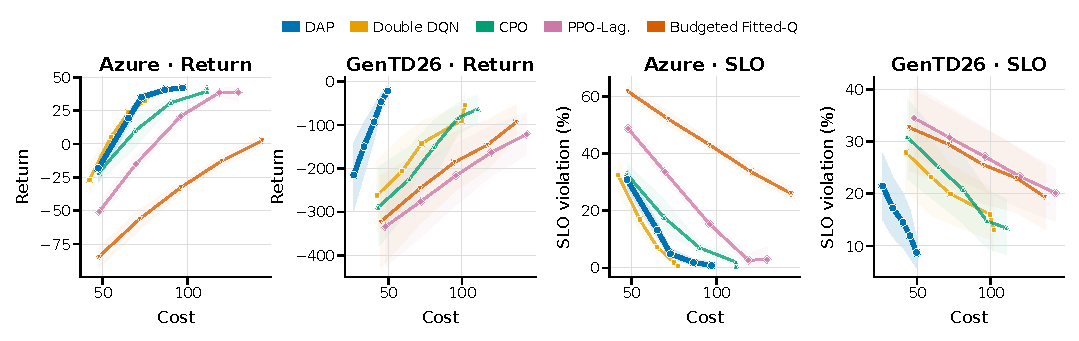
\includegraphics[width=.99\textwidth]{figures/F1_public_workload_frontiers.pdf}
  \caption{Public-workload service--cost frontiers.  The first two panels show
  return (higher is favorable) and the last two show SLO violation (lower is
  favorable), each against observed cost for Azure and GenTD26.
  Each point is one registered budget averaged over ten independently trained
  seeds; translucent ribbons are seed-bootstrap 95\% intervals for the
  vertical endpoint, and lines connect observed budgets only.}
  \Description{Four trend panels compare return and SLO violation against cost
  on Azure and GenTD26. A shared color-block legend
  identifies DAP and four ordinary, constrained, and budgeted RL baselines.}
  \label{fig:frontier}
\end{figure*}

Figure~\ref{fig:external-effects} reports the corresponding paired effects
after averaging budgets within each trained seed.

\begin{figure*}[t]
  \centering
  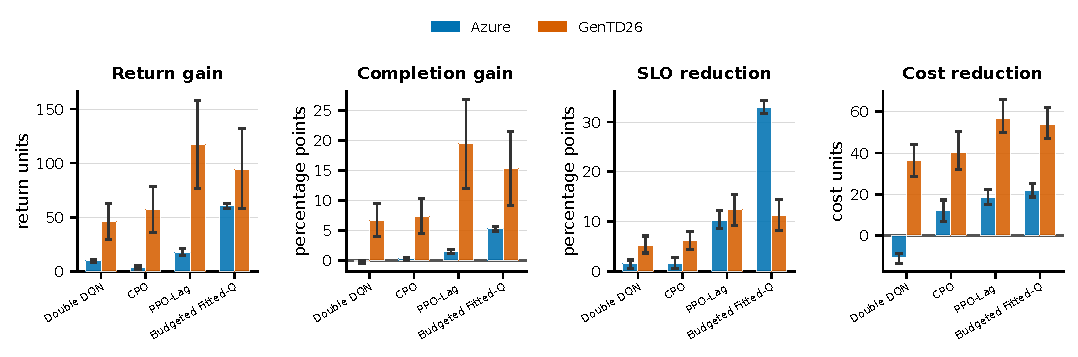
\includegraphics[width=.99\textwidth]{figures/F3_paired_external_effects.pdf}
  \caption{\textbf{DAP improvement over baseline.}  Define
  \(\Delta R=R_{\mathrm{DAP}}-R_{\mathrm{baseline}}\) and
  \(\Delta C=C_{\mathrm{DAP}}-C_{\mathrm{baseline}}\); SLO reduction is
  \(\mathrm{SLO}_{\mathrm{baseline}}-\mathrm{SLO}_{\mathrm{DAP}}\), and cost
  reduction is \(\mathrm{Cost}_{\mathrm{baseline}}-\mathrm{Cost}_{\mathrm{DAP}}
  =-\Delta C\).  The four endpoints are therefore oriented so that positive
  bars favor DAP.  Whiskers are paired-bootstrap 95\% CIs over ten trained seed
  blocks after averaging five budgets; completion and SLO use percentage
  points, while return and cost retain native units.}
  \Description{Four grouped vertical-bar panels report return,
  completion, SLO, and cost effects for DAP against four baselines. Color
  blocks separate Azure and GenTD26, and upward bars favor DAP.}
  \label{fig:external-effects}
\end{figure*}

These results connect finite-budget planning to an operator's choice of
service--resource regime. On GenTD26, the DAP mean operating point improves
all four outcomes relative to every comparator. On Azure, DAP combines a
favorable return--SLO frontier with lower cost than CPO, while the DAP and
Double DQN points offer different allocations of service and resource.
The frontiers make this choice explicit across the evaluated budgets.

\subsection{RQ2: Mechanisms of Action Comparison}
\label{sec:mechanisms}

The mechanism study separates the representation of action effects from the
estimation of future value. Matched controls test these components on workload
traces, and an exhaustive dynamic-programming diagnostic directly measures
the resulting action order.

\paragraph{Explicit effects and continuation.}
Matched temporal controls cover all 100 dataset--budget--seed cells,
with the original checkpoints and matched windows. Table~\ref{tab:revision-trace}
shows that Azure DAP improves return, completion, and proxy SLO over immediate
planning and MPC-8 after correction. Against a learned full transition with
the same frozen continuation weight, both datasets improve on all four
endpoints. DAP's mean
decision times are 0.81/0.95 ms, versus 144.88/189.04 ms for MPC-8 in this run.

The budget/horizon comparison pairs a full-feature value model with a masked
model trained from the same initialization, data, batches, GPU, and selected
round. This pairing isolates the information available to the value model. Table~\ref{tab:revision-trace} reports this
paired control alongside the frozen-checkpoint comparisons. The learned
transition has width 96 and trains for 24 epochs; feature controls retain
18 FVI rounds, two epochs per round, and the frozen continuation weight.
Training uses PyTorch 2.11 on an RTX 5090; planning runs on CPU. Frozen selection chooses zero continuation in 8/50 Azure and
16/50 GenTD26 checkpoints; those cells reduce to immediate scoring.

\begin{table}[t]
\caption{Temporal mechanism controls over all five budgets and ten paired training seeds per dataset. Differences are DAP minus comparator; $\dagger$ instead compares the full-feature retrain with its identically initialized masked-feature counterpart. Return includes pointwise 95\% intervals; completion and SLO differences use percentage points. Stars indicate Holm-adjusted $p<.05$ within each fixed study family (24 trace, 16 learned-model, eight matched-feature endpoints).}
\label{tab:revision-trace}
\small
\begin{tabular}{llrrrr}
\toprule
Dataset & Comparator & $\Delta$ return [95\% CI] & $\Delta$ comp. & $\Delta$ SLO & $\Delta$ cost\\
\midrule
Azure & Immediate & $+8.72 [+7.32, +10.20]^{*}$ & $+1.11^{*}$ & $-4.52^{*}$ & $-3.46$\\
 & PDS/ADP & $+0.73 [-0.24, +1.62]$ & $+0.04$ & $-0.24$ & $-0.80$\\
 & MPC-8 & $+4.80 [+3.98, +5.68]^{*}$ & $+0.69^{*}$ & $-2.39^{*}$ & $-3.46$\\
 & Learned trans. & $+5.38 [+3.81, +7.01]^{*}$ & $+0.65^{*}$ & $-2.54^{*}$ & $-7.73^{*}$\\
 & No B/H$^\dagger$ & $+4.68 [+1.72, +8.10]$ & $+0.32$ & $-2.07$ & $-0.65$\\
\midrule
GenTD26 & Immediate & $+1.79 [-0.13, +4.25]$ & $+0.20$ & $-0.04$ & $-0.24$\\
 & PDS/ADP & $+0.47 [-0.58, +1.65]$ & $+0.07$ & $+0.04$ & $-0.00$\\
 & MPC-8 & $-0.82 [-2.51, +0.85]$ & $+0.08$ & $+0.22$ & $-0.07$\\
 & Learned trans. & $+19.30 [+11.48, +27.98]^{*}$ & $+3.79^{*}$ & $-2.07^{*}$ & $-19.09^{*}$\\
 & No B/H$^\dagger$ & $-1.91 [-9.11, +7.65]$ & $-0.65$ & $+0.25$ & $+7.26$\\
\bottomrule
\end{tabular}
\end{table}


\paragraph{Action-ordering accuracy.}
Exact DP supplies an exhaustive reference for the branch comparison by
evaluating every feasible state--budget--horizon--action tuple.

For state \(s\), budget \(b\), horizon \(h\), and candidate \(a\), backward DP
defines \(Q^\star(s,b,h,a)\) and regret
\(Q^\star(s,b,h,a^\star)-Q^\star(s,b,h,\hat a)\), with the lowest-index exact
maximizer \(a^\star\). True-transition, black-box, and structured branches
reach .9553/.8805/.9460 agreement and .0191/.0613/.0188 regret; the structured
branch reduces Q-star regret 69.33\% and large-regret errors 99.49\%.
Table~\ref{tab:dp} reports the exhaustive ordering diagnostic.

\begin{table}[t]
\caption{Exhaustive exact-DP action-ordering diagnostic over every feasible
state--budget--horizon--action tuple.  Lower Q-star regret is favorable.}
\label{tab:dp}
\small
\begin{tabular}{lrr}
\toprule
Planner branch & Action agreement & Q-star regret\\
\midrule
True transition + learned value & .9553 & .0191\\
Black-box learned transition & .8805 & .0613\\
Structured action effects & .9460 & .0188\\
\bottomrule
\end{tabular}
\end{table}

The diagnostic fixes horizon 16, arrivals \(\{1,2,4\}\), queues 0--6, budgets
0--12, costs \((0,1,2,3)\), capacities \((1,2,3,4)\), and \(\gamma=.99\),
with stable, burst, and periodic load scenarios. Backward DP evaluates the full
feasible state--budget--horizon--action grid over three scenarios and five seeds;
ties use the lowest action index.

The large-regret set is the upper quartile of positive Q-star regret among
black-box-model disagreements: threshold 0.7073, 1,365 states, and
1,365 versus seven errors for black-box and structured branches. The 69.33\% and
99.49\% are exhaustive-grid ratios, while bootstrap uncertainty is reported for
1,800 rollouts. This grid quantifies the ordering mechanism; workload-scale
behavior is reported in the trace and live evaluations, with independent paired
Kubernetes runs.

\paragraph{Alternative post-decision value representation.}
\label{sec:pds}

The preregistered PDS comparator tests a closely related value representation. It applies the exact
action, reward, queue, budget, and horizon transition, then removes next-load
fields before the exogenous value is revealed. The afterstate network scores
feasible actions as immediate reward plus discounted post-decision value. It
shares the frozen DAP backbones, data, widths, candidate rounds, continuation
weights, guardrails, budgets, and seeds; all development and temporal cells use
the same code and contract hashes and complete with zero overspend.

The methods select different actions in 3.69--13.47\% of Azure states and
1.09--4.11\% of GenTD26 states. Their complete temporal contrasts appear in
Table~\ref{tab:revision-trace}. The PDS adapter also provides a portability
test: the same execution interface carries a different value representation
while preserving its clean scores and actions. This separates the reusable
verification capability from the choice of continuation model.

The matched-transition and exact-DP results support the same interpretation:
exposing known action effects improves the ordering on which the controller
acts. Azure's continuation gains show how the post-cost value can further
improve service beyond immediate scoring. DAP obtains these gains with
sub-millisecond mean planning in the matched study, while the PDS adapter
demonstrates that the verification interface also accommodates an alternative
value representation.

\subsection{RQ3: Verification and Deployed Resource Control}
\label{sec:deployment}

RQ3 connects independent checks across DAP and PDS with live resource control.
Paired Kubernetes plans measure service outcomes, delivered commands, and
resource accounting through a real orchestration API.

\paragraph{Independent verification across representations.}
The contract makes relationships between software components executable.
To test this capability, a trace adapter injects faults before branch construction,
selection, mapping, delivery, or ledger updates take effect. The seven fault
types are stale cycle context, inconsistent forecast, incorrect post-cost
budget, nonmaximal selection, target remapping, delivery override, and omitted
ledger charge. The checker receives independently witnessed context and
actuator receipts without fault labels. For example, a recorded decision selects capacity
6 with score 1.801; a delivery override executes the valid, affordable capacity
5 with score 1.785. Local validity checks accept either target, while the
independent receipt exposes the change in planner-to-actuator identity.
All 640 clean DAP/PDS decision contexts preserve
the original scores and actions. On independently witnessed activated faults,
the cross-boundary checker detects and localizes 1,940/1,940 DAP and
1,614/1,614 PDS violations; local validity, bounds, and affordability assertions
detect 6/3,554, while passive logs perform no automatic detection. Clean
false positives are 0/640; median checker-only time is 7.80 microseconds
(95th percentile 8.69), excluding evidence collection and persistence.
A separate $+10\%$ coherent-capacity control yields 50 changed actions
in 640 contexts while preserving record consistency, and the checker
correctly retains those internally consistent records. Each injected run
executes one copied context; inactive cases and PDS forecast injections are
excluded from the applicable-fault denominator.
The executable specification is implemented through cross-boundary assertions,
with the same checks supporting both planning representations.

\paragraph{Matched live design.}
The matched study separates value, lookahead, and reserve effects by fixing the model and execution path and
pairing DAP, immediate scoring, MPC-4, and a 45-second DAP reserve at budgets
128 and 256, using ten request plans per profile (160 completed runs).
Plans map 32 consecutive trace bins to 32 five-second intervals using a
training-fitted rate conversion and ten fixed activity strata. Plan seeds are
2026100201--2026100210; method order rotates across seeds and reverses at the
second budget, whose order also alternates. Azure/GenTD26 use frozen
continuation weights 1/.05 and HTTP SLOs .25/1 seconds. MPC uses depth four
and zero terminal value; the 45-second arm changes DAP's mask reserve alone.
The shared kind node runs Kubernetes 1.35.1 and Python 3.11.6. Each worker
requests .25 CPU/96 MiB and is limited to one CPU/256 MiB, with one-second
readiness probes and a bounded queue/CPU-work HTTP service.

\begin{table}[t]
\caption{Matched live controls: means over ten paired plans, averaging budgets 128 and 256 within each plan. Completion and failure-or-SLO count all scheduled requests. Cost is sampled Ready-replica-seconds; binding is the percentage of decisions with a masked candidate. Full budget-specific results and all 18 corrected contrasts appear in the replication package.}
\label{tab:revision-live}
\small
\begin{tabular}{llrrrr}
\toprule
Profile & Method & Complete (\%) & Fail/SLO (\%) & Cost & Binding (\%)\\
\midrule
Azure & DAP & 92.98 & 61.10 & 61.98 & 0.00\\
Azure & Immediate & 86.22 & 53.27 & 135.93 & 19.69\\
Azure & MPC-4 & 88.56 & 47.96 & 133.13 & 14.53\\
Azure & DAP (45 s) & 92.90 & 60.62 & 56.88 & 57.66\\
\midrule
GenTD26 & DAP & 93.70 & 28.02 & 98.79 & 14.06\\
GenTD26 & Immediate & 89.05 & 37.24 & 82.34 & 10.62\\
GenTD26 & MPC-4 & 90.11 & 36.51 & 82.07 & 10.78\\
GenTD26 & DAP (45 s) & 92.74 & 36.42 & 78.99 & 66.72\\
\bottomrule
\end{tabular}
\end{table}


\paragraph{Service gains under matched execution.}
Table~\ref{tab:revision-live} holds the calibrated model and execution path
fixed. Averaged over both budgets within each of ten paired Azure plans, DAP
increases completion over immediate scoring by 6.77 points (95\% CI
[5.62, 7.88]) and reduces cost by 73.95 Ready-replica-seconds (CI
[-85.51, -62.96]), a 54.4\% saving. Against matched MPC-4, cost falls by
71.15 (CI [-85.86, -56.68]), or 53.4\%. All three effects have
Holm-adjusted $p=.0352$ across the fixed 18-endpoint family. A scheduling amendment resolved exact run identifiers and retained every
completed run; the interrupted preparation produced no requests or actions.
An eight-plan sensitivity omitting the two earlier plan seeds retains the
Azure completion--cost pattern (+6.79 points and -70.83 seconds versus immediate).
The 45-second control exposes the reserve's effect on the feasible set:
Azure/GenTD26 binding rises from 0/14.06\% to 57.66/66.72\%.
These comparisons show how continuation and the reserve shape different
parts of a decision: the former scores remaining opportunity, while the
latter determines which commands can be considered.

\paragraph{Execution fidelity and control cost.}
Across all 160 matched runs, 3,390,344 requests reconcile exactly and all 5,120
logged actions maximize their feasible score vectors with the specified target
mapping. Every sampled ledger recomputes exactly, with zero budget violations
or controller deadline misses. The complementary 260-run controller and
robustness studies verify 3,840 DAP decisions, request closure, and restored
base readiness. Their affordability mask activates in 33/120 controller runs
and 248 decisions, removing 606 candidate opportunities. A replay verifier
additionally localizes each of six single-field mutations in 3,200 decision
records (19,200/19,200), checking forecast equality, feasible argmax, delivery
identity, target mapping, affordability, and ledger closure.

The Kubernetes loop uses Prometheus telemetry, a five-second period, a
32-cycle horizon, and 128/256 Ready-replica-second ceilings. Mean
inference/full-loop times in the controller study are 0.98/0.90 ms and
0.248/0.282 s for Azure/GenTD26. The corresponding trace timing benchmark
measures 0.630/0.613 ms for DAP, 46.46/37.84 ms for MPC-4, and
181.24/142.23 ms for MPC-8; Section~\ref{sec:mechanisms} reports timing in
the matched mechanism study. The amortized value keeps online comparison
small relative to the control period. Deadline checks cover every run, and
the artifact records tail latency and controller resource use.

\paragraph{Controller operating points.}
In the scheduler comparison, Azure DAP raises completion by 7.97 points
(95\% CI [6.48, 9.52]) and reduces Ready cost by 49.53 replica-seconds
(CI [-64.75, -35.18]) over MPC-4. Under binding GenTD26, completion rises
3.68 points (CI [1.40, 6.15], Holm-adjusted \(p=0.0264\)), with a mean cost
difference of +0.049 (CI [-11.40, 10.39]). The two profiles provide service
gains at lower or nearly equal mean cost; SLO intervals accompany both.

MPC-4 and Threshold use settings selected on a disjoint 180-run screen.
The native-controller study evaluates DAP, HPA, and Kubernetes Event-Driven
Autoscaling (KEDA) on common frozen plans
(Table~\ref{tab:k8s-cross}).
Both use one to five replicas and zero scale-up/down stabilization. HPA
targets 65\% CPU with a two-Pod/10-second scale-up policy; KEDA polls
queue depth every 10 seconds, with threshold four, a 20-second cooldown,
and a two-Pod/5-second scale-up policy. Both allow 100\% scale-down per
five seconds. The native controllers reserve 45 seconds for recovery; DAP uses the calibrated
3.2768/3.2632-second guards. These rows describe the complete configured
service--resource operating points.

Table~\ref{tab:k8s-cross} exposes all service--resource operating points.
On Azure, DAP uses 35.96/71.21 fewer Ready-replica-seconds than HPA/KEDA,
with completion .9654 and latency-SLO violation .3705. GenTD26 DAP provides
a .9723-completion, .0690-SLO operating point at 227.17 Ready-replica-seconds.
The four paired cost contrasts have Holm-adjusted $p=.0234$; the service
means describe the configured operating points ($p=.0625$--$.2227$).

\begin{table}[t]
\caption{Direct native-controller comparison on the tested Kubernetes cluster
(means over ten paired plans). Cost is additional Ready-replica-seconds; SLO
uses the latency-only violation definition. Bold marks the favorable
value in each profile and column.}
\label{tab:k8s-cross}
\small
\begin{tabular}{llrrr}
\toprule
Profile & Method & Completion $\uparrow$ & SLO $\downarrow$ & Ready cost $\downarrow$\\
\midrule
Azure & DAP & \textbf{.9654} & \textbf{.3705} & \textbf{48.37}\\
Azure & HPA & .9490 & .6157 & 84.33\\
Azure & KEDA & .9520 & .4116 & 119.58\\
\midrule
GenTD26 & DAP & \textbf{.9723} & \textbf{.0690} & 227.17\\
GenTD26 & HPA & .8265 & .2002 & 96.46\\
GenTD26 & KEDA & .8727 & .2440 & \textbf{59.81}\\
\bottomrule
\end{tabular}
\end{table}


\paragraph{Lifecycle calibration and sensitivity.}
The deployed controller uses startup-derived guards \(G=3.2768\) seconds
(Azure) and \(3.2632\) seconds (GenTD26). A direct lifecycle study measures 60
scale-up/return-to-base pairs across both profiles and targets 2, 3, and 5.
For each profile--target combination, the first five repetitions calibrate the maximum observed
Ready-withdrawal delay plus its sampling gap and a one-second margin; the next
five validate that rule. The resulting guards are 3.068/3.015 seconds, and all
30 validation withdrawals fit them (maxima 1.847/1.867 seconds). Pod deletion
is measured separately (maxima 2.530/2.549 seconds). These measurements use one
shared node under background activity. The paired
runs use the larger startup-derived guard
and continue accounting through observed return to base.

DAP preserves its registered service bounds under deterministic 10\%
sample-and-hold dropout on both profiles, while the independent Ready channel
remains intact. Across dropout, one-cycle observation lag, and five-second
readiness delay, all 60 fault runs preserve deadline, delivery, cleanup,
restoration, and sampled-ledger invariants.

DAP remains stable when explicit action-effect estimates are perturbed. Across
96,000 chronological development decisions, \(\pm5\%\) changes at most 6.91\%
of actions and 0.56 completion points; \(\pm10\%\) changes 10.55\% and 0.62
points. The mask records zero trace-token overspend. This sensitivity characterizes the action-effect calibration used to
construct the branches.

\section{Discussion and Applicability}

The results support a software design principle: preserve explicit action
semantics where resource decisions are compared, delivered, and charged.
Matched-transition controls connect this structure to service productivity;
the PDS adapter demonstrates reusable verification across value
representations. An independently witnessed command can reveal a selection
discrepancy even when both targets are locally valid. The separate ledger
similarly connects admission to measured consumption. These relations help
locate selection, delivery, and accounting discrepancies at their software
boundaries.

Applying the contract requires an action-effect model, a resource ledger,
and an observable actuator. Trace scheduling uses exact token costs;
Kubernetes uses calibrated capacity, recovery timing, and sampled Ready
accounting. A new deployment calibrates these quantities while preserving
common-context, feasible-selection, and receipt checks. Under the conditions
in Section~\ref{sec:k8s}, the reserve connects each admitted command to its
return to base. Thus the interface transfers with workload- and
deployment-specific models and resource semantics.

Each evaluation supplies a distinct form of evidence. Paired trace seeds
measure service productivity; exact DP isolates action ordering; and paired
HTTP plans measure live service and Ready cost on the tested cluster.
Trace SLO measures describe the queue model, while live outcomes use request
receipts. Pairing and disjoint selection inputs make mechanism contrasts
interpretable within those conditions. Together, these designs separate
the quality of a resource decision from its preservation through execution.

\section{Related Work}

\paragraph{Autonomic control and cloud resource management.}
Autonomic software frames adaptation as a monitored feedback loop
\cite{kephart2003autonomic}. Cloud controllers combine queue models,
forecasting, and autoscaling: AutoControl, AutoScale, Autopilot, Sinan, and
Autothrottle cover virtualized capacity and microservice SLOs
\cite{padala2009autocontrol,gandhi2012autoscale,rzadca2020autopilot,
zhang2021sinan,wang2024autothrottle}. Recent FSE systems add knowledge loops,
predictive PID, content-aware signals, and LLM-assisted Kubernetes operations
\cite{sanwouo2025aware,xiao2025tepid,duan2026aims,vitui2026aiops}. They expose
state and commands, whereas DAP records candidate consequences, budget
commitment, comparable scores, delivered command, and actuator/ledger evidence.
Kubernetes separates desired state, readiness, and reconciliation
\cite{burns2016kubernetes,kuberneteshpa,kubernetesprobes}; DAP makes the
resulting boundaries auditable through forecast equality, feasible selection,
target mapping, delivered identity, and ledger closure.

\paragraph{Cluster scheduling and learned policies.}
Cluster and serving systems optimize placement, packing, interference, and tail
behavior \cite{hindman2011mesos,schwarzkopf2013omega,vavilapalli2013yarn,
verma2015borg,delimitrou2013paragon,delimitrou2014quasar,grandl2014tetris,
grandl2016graphene,gog2016firmament,crankshaw2017clipper,
gujarati2020clockwork,alipourfard2017cherrypick,shahrad2020serverless,
akkus2018sand,oakes2018sock,kaffes2019core,dean2013tail}. DeepRM and Decima
learn policies from interaction, while constrained methods add costs, trust
regions, Lyapunov bounds, or penalty updates
\cite{mao2016deeprm,mao2019decima,altman1999cmdp,achiam2017cpo,
tessler2019rcpo,stooke2020pid,chow2018lyapunov,zhang2022p3o}. Budgeted RL
and LCPO address available budgets and changing contexts
\cite{carrara2019budgeted,hamadanian2025lcpo}. DAP complements these policy and value representations with explicit
branch provenance, hard affordability, and planner-to-actuator identity.

\paragraph{Planning, post-decision value, and action ordering.}
Dyna, MPC, and ADP combine learning, constrained search, and value approximation
\cite{sutton1991dyna,mesbah2016smpc,
powell2011adp}. Post-decision-state methods separate the action-controlled
transition from subsequent exogenous uncertainty and can impose structural
value properties \cite{jiang2015monotoneadp,bhat2026pds}. DAP carries this
decomposition into deployment: every affordable candidate receives one causal
realization, an explicit post-cost state and score, and a preserved identity
through argmax, actuation, and ledger closure. PDS/ADP and MPC isolate value
and search components, while exact DP measures ordering directly.

\section{Conclusion}

Direct Action Planning makes affordable action comparison an explicit
interface between learning and execution. Structured branches combine known
resource effects with post-cost continuation, while decision records connect
selection to actuation and accounting. Matched controls demonstrate resource
productivity and efficient planning; DAP/PDS checks establish reusable
verification; and Kubernetes runs demonstrate faithful deployment. Preserving
action semantics across these boundaries makes finite-budget scheduling both
effective and independently inspectable.

\clearpage
\section{Data Availability}

\begin{sloppypar}
The anonymous replication package is available at
\url{https://anonymous.4open.science/r/direct-action-planning-reproducibility-3642/}.
It contains source code, frozen checkpoints, trace preprocessing, configurations, controller
and environment definitions, and the manuscript's tables and figures. The
\texttt{evidence/} directory provides per-episode/per-plan outcomes, all 66
matched statistical contrasts, selected continuation weights, executable-fault
records, 60 lifecycle measurements, runtime versions, checksums, and a script
that recomputes the paired analyses. The main text specifies the methods,
metrics, experimental conditions, and principal results; the repository
provides the corresponding machine-readable evidence and detailed protocols.
Azure acquisition and GenTD26's pinned source, preprocessing recipe, and access
instructions are documented under \texttt{data/}; redistribution follows the
source datasets' terms. A public release will be maintained upon acceptance.
\end{sloppypar}

\bibliographystyle{ACM-Reference-Format}
\bibliography{references}

\end{document}
